\documentclass[conference]{IEEEtran}

\usepackage{cite}
\usepackage{amsfonts,amsmath,amssymb,amsthm,booktabs,color,enumitem,graphicx}


% correct bad hyphenation here
\hyphenation{op-tical net-works semi-conduc-tor}


\begin{document}

\title{Importance of software architecture in continuous deployment}

\author{\IEEEauthorblockN{Olli Rissanen}
\IEEEauthorblockA{Department of Computer Science\\
University of Helsinki\\
Helsinki, Finland\\
Email: olli.rissanen@helsinki.fi}}

% make the title area
\maketitle


\begin{abstract}
%\boldmathC
Currently more and more software companies are moving to lean practices, which often include shorter delivery cycles and thus shorter feedback loops. However, to achieve continuous customer feedback and to eliminate work that doesn't generate value, even shorter cycles are required. In continuous deployment the software functionality is deployed continuously at customer environment. This process includes both automated builds and automated testing, but also automated deployment. This adds more elements to the development pipeline, which often in a lean team consists of a version control system and a continuous integration server. Automating the whole process minimizes the time required for implementing new features in software, and allows for faster customer feedback. In this paper we review the importance of architecture in development pipelines that implement continuous deployment. We investigate the challenges a company typically faces during the transition to continuous deployment. We also explore the main issues and attributes required for the architecture of the the pipeline to allow gathering feedback in real-time. We aim for a coherent view of essential features required to build a development pipeline in such manner. 
\end{abstract}
% IEEEtran.cls defaults to using nonbold math in the Abstract.
% This preserves the distinction between vectors and scalars. However,
% if the conference you are submitting to favors bold math in the abstract,
% then you can use LaTeX's standard command \boldmath at the very start
% of the abstract to achieve this. Many IEEE journals/conferences frown on
% math in the abstract anyway.

% no keywords




% For peer review papers, you can put extra information on the cover
% page as needed:
% \ifCLASSOPTIONpeerreview
% \begin{center} \bfseries EDICS Category: 3-BBND \end{center}
% \fi
%
% For peerreview papers, this IEEEtran command inserts a page break and


% creates the second title. It will be ignored for other modes.
\IEEEpeerreviewmaketitle

%Perusteet

%Kiinnostava
%Innostava
%Tehtävissä

%Määrittele
%	Tutkimusongelma, siis mitä haluat ymmärtää tai selvittää
%	Tavoitteet
%	Menetelmät
%	Rajaus

%Mahdollisia toteutustapoja
%	Vertaile kahta tai useampaa lähestymistapaa
%	Etsi empiiristä todistusaineistoa jonkin väitteen puolesta tai sitä vastaan
%	Kuvaa tapausyrityksen tilanne ja vertaile kirjallisuuteen
%

%Haasteet

%In fact, one sign of a good application architecture is that it allows the application
%to be run without much trouble on a development machine.

\section{Introduction} %why is this problem interesting?

Continuous deployment is an extension to continuous integration, where the software functionality is deployed frequently at customer environment. While continuous integration defines a process where the work is automatically built, tested and frequently integrated \cite{fowler2006continuous}, often multiple times a day, continuous deployment adds automated acceptance testing and deployment. The purpose of continuous deployment is that as the deployment process is completely automated, it reduces human error, documents required for the build and increases confidence that the build works \cite{cdbook}. 

In an agile process software release is done in periodic intervals \cite{cockburn2002agile}. Compared to waterfall model it introduces multiple releases throughout the development. Continuous deployment, on the other hand, attemps to keep the software ready for release at all times during development process \cite{cdbook}. Instead of stopping the development process and creating a build as in an agile process, the software is continuously deployed to customer environment. This doesn't mean that the development cycles in continuous deployment are shorter, but that the development is done in a way that makes the software always ready for release.

It should also be made clear that continuous delivery differs from continous deployment. Refer to Fig. \ref{fig1} for a visual representation of differences in continuous integration, delivery and deployment. Both include automated deployment to a staging environment. Continuous deployment includes deployment to a production environment, while in continuous delivery the deployment to a production environment is done manually. The purpose of continuous delivery is to prove that every build is proven deployable \cite{cdbook}. While it necessarily doesn't mean that teams release often, keeping the software in a state where a release can be made instantly is often seen beneficial.

In this paper we investigate the importance of software architecture, and especially architectural challenges required for the software to enable continuous deployment. In an agile process software architecture is often ignored, citing You Ain't Gonna Need It (YAGNI) and big-up front design (BUFD) \cite{kruchten2010software}, but in a process with continuous deployment architecture is especially important. An important research question regarding continuous delivery, posed by Akerele et al., is to investigate the variables in software projects that have a significant impact on the frequent delivery \cite{6612879}. Software architecture is one of the technological factors that affect the stability of the process. 

%why?
Important architectural qualities considering continuous delivery are especially extensibility and flexibility, which are better defined in \cite{kaisler2005software}. Extensibility covers the future growth, which in an incremental development process such as continuous deployment is a primary concern. Due to an extensible architecture flexibility is also provided.

As research on software architecture in continuous deployment is next to nonexistent, other areas of research have to be reviewed and applied to continuous deployment. Such areas are for example architectural challenges in agile development \cite{kruchten2010software} and analysis and management of architectural dependencies in iterative release planning \cite{brown2011analysis}. Especially useful are also the research in importance of software architecture during release planning \cite{lindgren2008importance} and software release management \cite{van1997software}.
The research on these topics can then be applied to continuous deployment, and along with the principles for continuous deployment \cite{humble2006deployment} combined into a coherent view of architectural challenges and features. 

Continuous deployment process is concerned with all aspects of deployment, such as configuration management, release management, continuous integration and automated testing. As it has evolved from continuous improvement efforts within the Agile community, but also from prior knowledge on releasing software, it is only natural to investigate these subjects to gain understanding on continuous deployment.

This paper is organized as follows. Chapter 2 explains reasons behind choosing the used papers, and the used methods in finding the papers. Chapter 3 explores architectural challenges and methods in release management, release planning and iterative release planning. Chapter 3 also investigates the deployment production line and the known architectural constraints within. Chapter 4 then attempts to apply these findings to continuous deployment, and produces an analysis of the importance of architecture in continuous deployment. Chapter 5 concludes the paper with key points.  

\begin{figure}[!t]
	\centering
	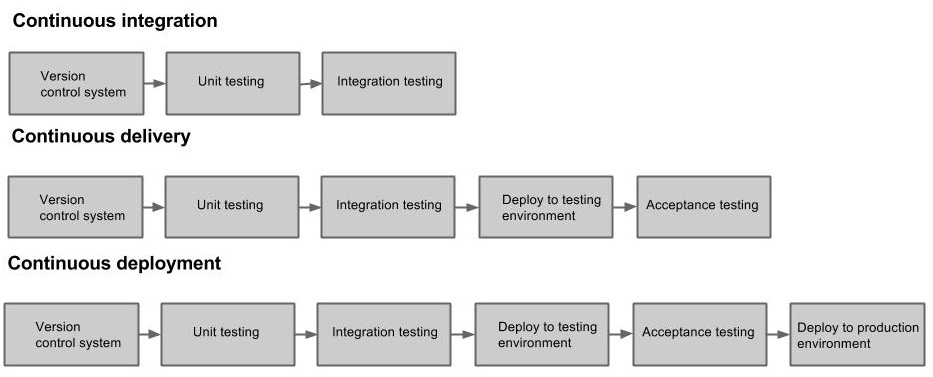
\includegraphics[width=3.5in]{rtvd.jpg}
	\caption{Continuous integration, delivery and deployment.}
	\label{fig1}
\end{figure}

\section{Methods} %how did I find the papers?

As continuous deployment is a relatively new area of research, all aspects of it have not yet been investigated. To better understand the architectural challenges in continuous deployment, it is important to research architectural challenges of processes with relations to continuous deployment.

Searches were performed using the keywords shown in Table 1. The searches were performed during February and March 2014 using IEEE Xplore (http://ieeexplore.ieee.org/‎) and Google Scholar (http://scholar.google.com/) search engines. Final papers were downloaded from the publishers web sites, if available. Alot of research concerning software release management, release planning and iterative release planning were found, but the focus on architectural qualities appeared sparsely.  

\begin{center}
    \begin{tabular}{ | p{2cm} | p{2cm} | p{3.5cm} |}
    \hline
    Search string & Search engine & Article \\ \hline
    software release management & Google Scholar & Software Release Management \\ \hline
	release planning architecture & IEEE Xplore & Importance of Software Architecture during Release Planning \\ \hline
	deployment production line & IEEE Xplore & The deployment production line \\ \hline
	iterative release planning architecture & IEEE Xplore & Analysis and Management of Architectural Dependencies in Iterative Release Planning \\ \hline
    \end{tabular}
\end{center}

As searches regarding architecture in continuous delivery and deployment returned no results, a decision was made to instead focus on research related to architectural features and issues in releases, and then attempting to apply those findings to continuous deployment. Articles regarding release management, release planning, iterative release planning and deployment pipeline were chosen for this purpose.

%Hoek et al. investigate management of software releases in their article Software Release Management \cite{van1997software}. 
%In the article Importance of Software Architecture during Release Planning \cite{lindgren2008importance}, which was presented in Seventh Working IEEE/IFIP Conference on Software Architecture, %Lindgren et al. investigate how architectural issues are considered during release planning in industry today. As continuous deployment is deals with continuous releases, the architectural %findings can be adapted to continuous deployment.

\section{Results} %Pure analysis on the papers
Release planning primarily plans releases that often occur months out at the start of a project. Iterative release planning on the other hand plans releases for the current iteration, which depending on the team could last from a week to four weeks. Release management is a process of managing often complex and distributed releases throughout development stages to release. In continuous deployment the challenge is to continuously keep the software in a state where it can be released. 

This section investigates the architectural issues and features in release management, release planning and iterative release planning, along with some known architectural issues and features in continuous deployment. The knowledge from previous research on release planning proves useful considering continuous deployment, as it is effectively continuously managing to maintain the software in a releasable state.

\subsection{Software release management}

Software release management defines the process of managing software releases throughout development stages to release. Compared to continuous deployment, release managements purpose is to build a bridge between development process and deployment process \cite{van1997software}, but it doesn't define how often releases should be made. Hoek et al. provide a set of requirements in their article Software Release Management \cite{van1997software}, which can be used to define architectural qualities in software systems required for releases. While the article mainly touches releases of systems of systems, the research can also be applied to releases of any systems with internal or external dependencies.

A requirement states that "Dependencies should be explicit and easily recorded". Hoek et al. define the requirement such that it should be possible for a developer to document dependencies as part of the release process, even if the dependencies cross organizational boundaries. Another requirement is that "A system should be available through multiple channels". This means that once a release is made, it is made available to all environments where it is used. A requirement also states that "Sufficient descriptive information should be available". This makes it possible for an user to determine the current version of system in use.

Hoek et al. introduce a prototype software release management tool, Software Release Manager (SRM), which is used to satisfy previous requirements. SRM is composed through a four-part architecture: a logically centralized but physically distributed release database, interfaces for inserting and retrieving components from the database and a retrieve database that records information about the components users have retrieved. 

\subsection{Release planning}

Lindgren et al. investigate the importance of software architecture in release planning in their article entitled Importance of Software Architecture during Release Planning \cite{lindgren2008importance}. Lindgren et al. state that within the research community it is known that early design decisions, which are manifested by software architecture, "...are the most difficult to get correct and the hardest to change later in the development process, and they have the most far-reaching effects" \cite{bass2003software}.

Lindgren et al. define relevant areas that address software architecture in release planning as identifying possible architectural constraints, maintaining the architecture of evolving systems and identifying if proposed needs introduce architectural conflicts. 

The major findings of the articles are that product management generally has low architectural awareness, there is no method for how to balance investments in quality improvements vs. feature growth and that in companies with a software architecture present architectural decisions are made with less "gut-feeling".

\subsection{Architectural Dependencies in Iterative Release Planning}

Iterative release planning essentially attemps to plan releases for the current iteration. Brown et al. investigate dependencies between capabilities, including both functional and non-functional requirements, and architectural elements \cite{brown2011analysis}. Brown et al. state that understanding the dependencies between capabilities ensures that a useful feature set is released to the end user. The purpose in investigating the dependencies between capabilities and architectural elements is to implement the architecture in a staged manner. Analysing the dependencies of architectural elements provides information on the refactoring costs that might incur if the architecture is developed incrementally.

Brown et al. state that the visibility of architectural quality can be improved by providing quantifiable quality models of the architecture module structure during system development. This derives from the assumption that using measurable criteria to quantify architecture quality provides guidance for iterative release planning.

Brown et al. calculate end-user value and total implementation cost of each release as $Tc_n = Ic_n + Rc_n$, where $Tc_n$ is the cost of release $n$, $Ic_n$ is the cost of implementation and is a sum of all architectural elements implemented in release $n$, where each architectural elements are given an individual cost. $Rc_n$ is the rework cost for release $n$, and it is calculated by computing the rework cost associated with each new architectural element implemented in $n$, and multiplying for each existing element with dependencies to that element times the implementation cost of the referencing element, times the propagation cost of release $n-1$. The cost of each element is then added up to form $Rc_n$.

\subsection{Deployment production line}

Humble et al. define four principles that should be followed when attempting to automate the deployment process \cite{humble2006deployment}. Some of these principles transform into architectural constraints. The first principle states that "Each build stage should deliver working software". As software often consists of different modules with dependencies to other modules, a change to a module could trigger builds of the related modules as well. Humble et al. argue that it is better to keep builds separate so that each discrete module could be built individually. The reasons to th is are that triggering other builds can be inefficient, and information can be lost in the process. The information loss is due to the fact that connection between the initial build and later builds is lost, or at least causes a lot of unnecessary work spent in tracing the triggering build. 

The second principle states that "Deploy the same artifacts in every environment". This creates a constraint that the configuration files must be kept separate, as different environments often have different configurations. Humble et al. state that a common anti-pattern is to aim for 'ultimate configurability', and instead the simplest configuration system that handles the cases should be implemented.

Another principle, which is the main element of continuous deployment, is to "Automate testing and deployment". Humble et al. argue that the application testing should be separated out, such that stages are formed out of different types of tests. This means that the process can be aborted if a single stage fails. They also state that all states of deployment should be automated, including deploying binaries, configuring message queues, loading databases and related deployment tasks. Humble et al. mention that it might be necessary to split the application environment into $slices$, where each slice contains a single instance of the application with predetermined set of resources, such as ports and directories. Finally, the environment can be smoke tested.

The last principle states "Evolve your production line along with the application it assembles". Humble et al. state that attempting to build a full production line before writing any code doesn't deliver any value, so the production line should be built and modified as the application evolves. 

\section{Discussion} %Own speculation

In continuous deployment it is preferred not to do huge refactorings due to the fact that this leaves the software in a state where it cannot be released /cdbook

In continuous deployment the architecture is developed incrementally, and this poses many similarities to iterative release planning.


The goal of the development process is to maximize business value. Using the cost model \cite{brown2011analysis} by Brown et al., 

As software release management is primarily concerned in .. \cite{van1997software} 

In release planning it is known that early design decisions play an important role in the development process \cite{lindgren2008importance}. As an example in a system with a high performance requirement, requests shouldn't traverse through several tiers. In a continuous deployment process, enough analysis on non-functional requirements has to be made up front to make an informed decision on what architecture to choose for the system \cite{cdbook}. Often an architecture also involves trade-offs between non-functional requirements, and analysis methods such as the Architectural Tradeoff Analysis Method (ATAM) \cite{kazman1998architecture} can be used to decide a suitable architecture. The team can then build a set of automated tests to ensure the non-functional requirements are met, and that empirical evidence to refactor and rearchitect a project is provided \cite{cdbook}.

"one good sign of a good application architecture is that it allows the application to be run without much trouble on a development machine"

The requirement "Each build stage should deliver working software" by Humble et al. \cite{humble2006deployment} creates an architectural requirement, in which each component should be possible to be upgraded individually. The same principles apply to individual services that form a service-oriented architecture \cite{cdbook}. A component-based architecture with loose coupling makes it easier for teams to develop and collaborate, especially in cases where the team sizes are large and codebases big. A component-based architecture is also effectively flexible, as components can be added and removed with often only having to modify related components. A decision to build the software in components should be made early on, as the time it takes to rearchitecture a large application into discrete components increases as the application grows. 

As continuous deployment keeps the software in a state where it can be deployed at all times, incomplete features often pose architectural challenges in keeping the build stable. Shipping semicompleted functionality along with the rest of the application is a good practice, because the entire application is tested and integrated at any time \cite{cdbook}. To implement the application in such manner that features can be included even if they are incomplete requires an architecture that supports it. A common tradition in an agile process is to use branching in version control to develop features, but with the possibility to build the application with incomplete features allows releases even during the development of major features. 

An architectural quality regarding continuous deployment is also the architecture of the whole development process. A picture of the typical development process in continuous deployment is shown in Fig. 2. After the team pushes a change to the version control system, the project is automatically built and tests are triggered stage by stage. If a test stage fails, feedback is given and the deployment process effectively cancelled. In a continuous delivery process, the last stages are approved and activated manually, but in a continuous deployment process the last stages are triggered automatically as well.

\begin{figure}[!t]
	\centering
	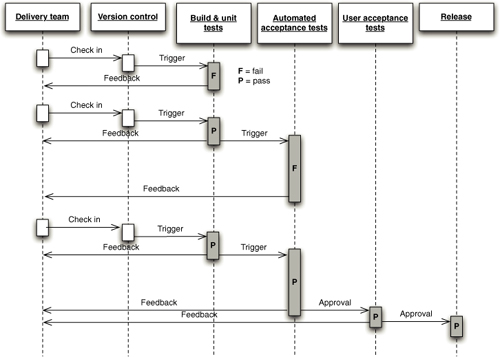
\includegraphics[width=3.5in]{developmentprocess.jpg}
	\caption{Architecture of the development process \cite{cdbook}.}
	\label{fig1}
\end{figure}

\subsection{Further research questions}


asd


early design decisions, manifested by the software architecture,
“. . . are the most difficult to get correct and the hardest to
change later in the development process, and they have the
most far-reaching effects”


research questions

When and how are architectural issues addressed during release planning? \cite{lindgren2008importance}

%How the previous stuff actually matters to continuous deployment

\section{Conclusion} %Short wrap-up. Contains the key points
% no \IEEEPARstart

In a continuous deployment process, enough analysis on non-functional requirements has to be made up front to make an informed decision on what architecture to choose for the system.

A component-based architecture, such as a service-oriented architecture, generally makes the developing and building easier.


%ASD
Architectural problems:
maven snapshot release builds http://kief.com/the-conflict-between-continuous-delivery-and-traditional-agile.html

rearchitecting

testing.
Promoting Configuration
%In terms of implementation, NFRs are complex because they usually have a
%very strong influence on the architecture of the system. For example, any system
%that requires high performance should not involve requests traversing several
%tiers. Since the architecture of the system is hard to change later on in the delivery
%process, it is essential to think about nonfunctional requirements at the beginning
%of the project. This means doing just enough analysis up front to make an
%informed decision on what architecture to choose for the system.
%Every architecture involves some trade-off between nonfunctional
%requirements—

In the case of service-oriented architectures and componentized applications,
all the services or components forming the application need to be promoted together.
As we discussed in the previous section, it is usually in the system integration
testing environment that a good combination of versions of the application’s
services and components is found. Your deployment system needs to enforce that
this combination is then promoted as a whole, to avoid a situation where someone
deploys a wrong version of one of the services, causing the application to fail—or
worse, introducing an intermittent and hard-to-track-down defect.

%"Use the Same Scripts to Deploy to Every Environment"
If your application is complex in terms of its deployment architecture, you will
have to make some simplifications to get it working on developer machines.

benefits:
It doesnt take until release to notice that the softwares architecture doesn't support the systems nonfunctional requirements
%//ASD


% wat It has to be flexible enough to allow modifica


\bibliography{IEEEabrv,references}{}
\bibliographystyle{IEEEtran}
% trigger a \newpage just before the given reference
% number - used to balance the columns on the last page
% adjust value as needed - may need to be readjusted if
% the document is modified later
%\IEEEtriggeratref{8}
% The "triggered" command can be changed if desired:
%\IEEEtriggercmd{\enlargethispage{-5in}}

% references section

% can use a bibliography generated by BibTeX as a .bbl file
% BibTeX documentation can be easily obtained at:
% http://www.ctan.org/tex-archive/biblio/bibtex/contrib/doc/
% The IEEEtran BibTeX style support page is at:
% http://www.michaelshell.org/tex/ieeetran/bibtex/

% argument is your BibTeX string definitions and bibliography database(s)
%\bibliography{IEEEabrv,../bib/paper}
%
% <OR> manually copy in the resultant .bbl file
% set second argument of \begin to the number of references
% (used to reserve space for the reference number labels box)
%\begin{thebibliography}{1}

%\bibitem{IEEEhowto:kopka}
%H.~Kopka and P.~W. Daly, \emph{A Guide to \LaTeX}, 3rd~ed.\hskip 1em plus
%  0.5em minus 0.4em\relax Harlow, England: Addison-Wesley, 1999.

%\end{thebibliography}




% that's all folks
\end{document}


